% =====================================================================
% Figure: Three-regime phase transition from Theorem 1.
% Closes editorial decision item C-DA1 (formalises the IGNN-only scope).
% =====================================================================
%
% Compile standalone:
%   pdflatex -interaction=nonstopmode -halt-on-error fig_phase_transition.tex
%
% Include in paper as:
%   \begin{figure}[t]
%     \centering
%     
\includegraphics[width=\columnwidth]{figures/fig_phase_transition.pdf}
%     \caption{...}
%     \label{fig:phase_transition}
%   \end{figure}

\documentclass[tikz,border=4pt,11pt]{standalone}
\usepackage[T1]{fontenc}
\usepackage{mathptmx}  % Times-like serif text + math
\usepackage{tikz}
\usepackage{pgfplots}
\pgfplotsset{compat=1.18}
\usetikzlibrary{patterns, fillbetween, calc, decorations.pathreplacing}
\usepackage{xcolor}
\usepackage{amsmath, amssymb}
\renewcommand{\familydefault}{\rmdefault}

\definecolor{csub}{HTML}{009E73}      % green — subcritical (formal guarantees hold)
\definecolor{ccrit}{HTML}{F0E442}     % yellow — critical
\definecolor{csup}{HTML}{D55E00}      % vermilion — supercritical (theorem void)
\definecolor{cresolvent}{HTML}{0072B2}% blue — resolvent norm
\definecolor{cempkappa}{HTML}{555555} % grey — empirical kappa range

% Custom TikZ macros for the manual legend below the axis. Bypassing
% pgfplots' \addlegendimage system because per-entry `legend image code`
% overrides were silently ignored in this pgfplots version, causing entry 2
% and 3 to render with the wrong glyphs (both solid lines).
\newcommand{\legline}[1]{%
  \tikz[baseline=-0.55ex]{\draw[cresolvent, line width=0.9pt, #1]
        (0,0) -- (0.42cm, 0);}}
\newcommand{\legband}{%
  \tikz[baseline=-0.55ex]{%
    \fill[cempkappa, fill opacity=0.32] (0,-0.09) rectangle (0.42cm, 0.11);%
    \draw[cempkappa!55!black, line width=0.3pt]
        (0,-0.09) rectangle (0.42cm, 0.11);}}

\begin{document}
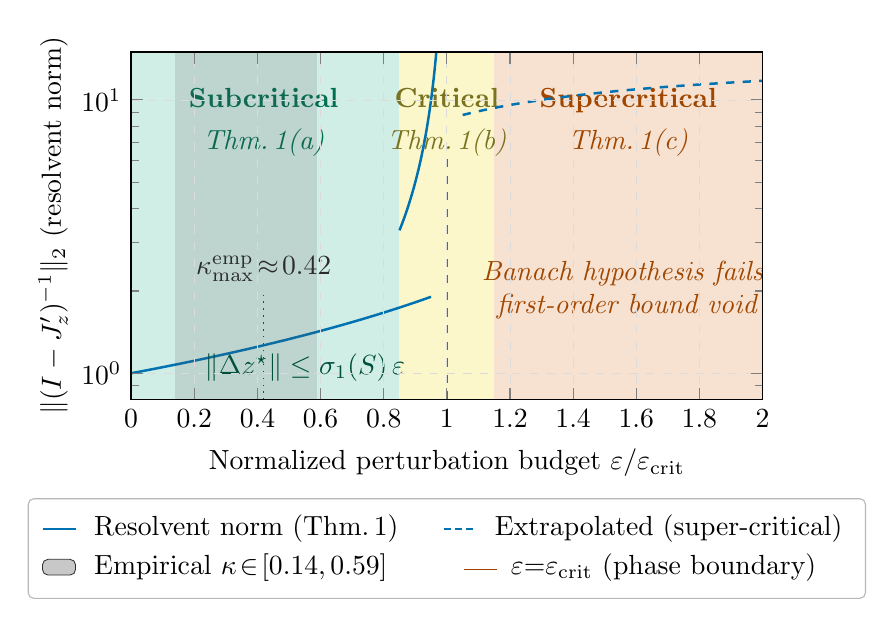
\begin{tikzpicture}[font=\rmfamily]
\begin{axis}[
    width=9.6cm, height=6.0cm,
    xmin=0, xmax=2.0,
    ymin=0.8, ymax=15,
    ymode=log,
    log basis y=10,
    xlabel={Normalized perturbation budget $\varepsilon / \varepsilon_{\mathrm{crit}}$},
    ylabel={$\|(I - J_z')^{-1}\|_2$ (resolvent norm)},
    xlabel style={font=\rmfamily\normalsize, yshift=-1pt},
    ylabel style={font=\rmfamily\normalsize, yshift=-2pt},
    tick label style={font=\rmfamily\normalsize},
    grid=major, grid style={dashed, gray!28, line width=0.3pt},
    axis line style={line width=0.5pt},
    tick style={line width=0.4pt},
    axis on top,
    clip=true,
]

% --- Background regions ---------------------------------------------------
\fill[csub!18]   (axis cs:0,       0.8) rectangle (axis cs:0.85,  15);
\fill[ccrit!28]  (axis cs:0.85,    0.8) rectangle (axis cs:1.15,  15);
\fill[csup!18]   (axis cs:1.15,    0.8) rectangle (axis cs:2.0,   15);

% Region labels at the TOP of each region (out of curve's way)
\node[anchor=north, font=\rmfamily\normalsize\bfseries, text=csub!70!black]
     at (axis cs:0.42, 12) {Subcritical};
\node[anchor=north, font=\rmfamily\normalsize\itshape, text=csub!70!black]
     at (axis cs:0.42, 8.5) {Thm.\,1(a)};
\node[anchor=north, font=\rmfamily\normalsize\bfseries, text=ccrit!50!black]
     at (axis cs:1.00, 12) {Critical};
\node[anchor=north, font=\rmfamily\normalsize\itshape, text=ccrit!50!black]
     at (axis cs:1.00, 8.5) {Thm.\,1(b)};
\node[anchor=north, font=\rmfamily\normalsize\bfseries, text=csup!75!black]
     at (axis cs:1.575, 12) {Supercritical};
\node[anchor=north, font=\rmfamily\normalsize\itshape, text=csup!75!black]
     at (axis cs:1.575, 8.5) {Thm.\,1(c)};

% --- Resolvent norm: simplified worst-case 1/(1-x) family ----------------
\addplot[
    cresolvent, line width=0.9pt, smooth, samples=80,
    domain=0:0.95, name path=resolvent_lo,
]
{1 / (1 - 0.5 * x)};
\addplot[
    cresolvent, line width=0.9pt, smooth, samples=80,
    domain=0.85:0.999, name path=resolvent_hi,
]
{0.5 / (1 - x)};
\addplot[
    cresolvent, line width=0.9pt, dashed, samples=50,
    domain=1.05:2.0,
] {15 - 6.5/x};

% --- Empirical kappa range band: [0.14, 0.59] ---------------------------
\addplot[draw=none, fill=cempkappa, fill opacity=0.16, forget plot]
    coordinates {(0.14, 0.8) (0.59, 0.8) (0.59, 15) (0.14, 15)};

% (Empirical kappa range is now described in the legend; in-plot label removed
%  to avoid duplication and free up bottom-subcritical white space.)

% --- Vertical line at eps = eps_crit (label moved to legend; arrow kept here)
\draw[csup!85!black, line width=0.8pt, dashed]
     (axis cs:1, 0.8) -- (axis cs:1, 6.5);
% Empirical saturation marker at kappa ~ 0.42 (paper text Sec. Phase Transition)
\draw[cempkappa!75!black, line width=0.5pt, dotted]
     (axis cs:0.42, 0.8) -- (axis cs:0.42, 2.0);
\node[anchor=south, font=\rmfamily\normalsize, text=cempkappa!50!black]
     at (axis cs:0.42, 2.0) {$\kappa_{\max}^{\mathrm{emp}}\!\approx\!0.42$};

% --- First-order bound annotation in subcritical region -----------------
\node[anchor=center, font=\rmfamily\normalsize, text=csub!50!black]
     at (axis cs:0.55, 1.05) {$\|\Delta z^\star\|\le\sigma_1(S)\,\varepsilon$};

% --- Supercritical: theorem void (kept far inside the supercritical region) -
\node[anchor=south, font=\rmfamily\normalsize\itshape,
      text=csup!75!black, align=center]
     at (axis cs:1.57, 1.45) {Banach hypothesis fails;\\first-order bound void};

\end{axis}

% --- Manual two-row legend, placed BELOW the axis (outside the plot area).
%     Drawn with plain TikZ + a 2-column tabular so glyphs (solid line /
%     dashed line / filled rectangle) render deterministically and the
%     legend's width is roughly half the single-row version. Two rows save
%     horizontal whitespace and let the figure breathe vertically.
\node[anchor=north, font=\rmfamily\normalsize,
      draw=black!28, fill=white, rounded corners=2pt, inner sep=5pt,
      align=center]
    at ($(current axis.south) + (0, -1.25cm)$) {%
   \begin{tabular}{@{}l@{\hspace{6pt}}l@{\hspace{16pt}}l@{\hspace{6pt}}l@{}}
     \legline{solid} & Resolvent norm (Thm.\,1) &
     \legline{dash pattern=on 2.4pt off 1.6pt} & Extrapolated (super-critical) \\[2pt]
     \legband & Empirical $\kappa\!\in\![0.14,0.59]$ &
     \multicolumn{2}{l}{\textcolor{csup!75!black}{\,\rule[0.4ex]{0.42cm}{0.4pt}\,} $\varepsilon{=}\varepsilon_{\mathrm{crit}}$ (phase boundary)} \\
   \end{tabular}
};

\end{tikzpicture}
\end{document}
